\documentclass[10pt,twocolumn,letterpaper]{article}

\usepackage[review]{cvpr}
\usepackage{times}
\usepackage{epsfig}
\usepackage{graphicx}
\usepackage{amsmath}
\usepackage{amssymb}
\usepackage{booktabs}
\usepackage{multirow}
\usepackage{enumitem}
\usepackage[table]{xcolor}
\usepackage{colortbl}
\usepackage{tikz}
\usepackage{pgfplots}
\usepackage{rotating}
\pgfplotsset{compat=1.18}
\usetikzlibrary{shapes.geometric, arrows.meta, positioning, fit, calc, backgrounds, decorations.pathreplacing}
\usepackage[pagebackref=true,breaklinks=true,letterpaper=true,colorlinks,bookmarks=false]{hyperref}

% Space tightening — between aggressive and mild.
\setlength{\abovedisplayskip}{4.5pt plus 1pt minus 1pt}
\setlength{\belowdisplayskip}{4.5pt plus 1pt minus 1pt}
\setlength{\abovedisplayshortskip}{2pt plus 1pt}
\setlength{\belowdisplayshortskip}{2.5pt plus 1pt minus 1pt}
\setlength{\textfloatsep}{9pt plus 2pt minus 2pt}
\setlength{\floatsep}{7.5pt plus 2pt minus 2pt}
\setlength{\intextsep}{7.5pt plus 2pt minus 2pt}
\makeatletter
\renewcommand\section{\@startsection{section}{1}{\z@}%
  {-1.5ex \@plus -0.4ex \@minus -0.2ex}%
  {0.8ex \@plus 0.2ex}%
  {\normalfont\large\bfseries}}
\renewcommand\subsection{\@startsection{subsection}{2}{\z@}%
  {-1.2ex \@plus -0.4ex \@minus -0.2ex}%
  {0.5ex \@plus 0.2ex}%
  {\normalfont\normalsize\bfseries}}
\renewcommand\subsubsection{\@startsection{subsubsection}{3}{\z@}%
  {-0.8ex \@plus -0.3ex \@minus -0.2ex}%
  {0.4ex \@plus 0.2ex}%
  {\normalfont\normalsize\bfseries}}
\makeatother

\def\httilde{\mbox{\tt\raisebox{-.5ex}{\symbol{126}}}}

% Custom commands
\newcommand{\method}{\textsc{GenStack}}
\newcommand{\vfive}{\textsc{Pact}}
\newcommand{\prism}{\textsc{Prism-SFT}}
\newcommand{\rh}[1]{\rotatebox{60}{\small #1}}  % rotated header

\begin{document}

%%%%%%%%% TITLE
\title{GenStack: Dual-Branch Mixture of Experts for Generalizable Face Forgery Detection}

\author{Anonymous Authors\\
Anonymous Institution\\
{\tt\small anonymous@example.com}
}

\maketitle
\thispagestyle{empty}

% =====================================================================
% Abstract
% =====================================================================
\begin{abstract}
Face forgery detection is becoming harder as new generators continue to emerge, ranging from GAN-based face swaps to diffusion-driven relighting and fully AI-generated portraits. Most existing detectors are trained on a narrow set of generators and do not generalize well to unseen ones. Recent vision--language detectors further rely on a single backbone and a single RGB view, missing the spectral and noise-residual cues that often expose modern fakes. We present \textsc{GenStack}, a two-branch detector that combines complementary discriminative and reasoning-based signals. It pairs \textsc{Pact}, a parameter-efficient discriminative head built on a frozen CLIP ViT-L/14 with learnable forgery prompts and prototype-grounded attention, with \textsc{Prism-SFT}, an InternVL3-8B reasoner fine-tuned on RGB, frequency, and noise-residual views to produce a short region-grounded explanation before its verdict. We train $K$ small Gradient Boosting experts and combine them at inference via a lightweight learned soft gate built on CLIP features already extracted by \vfive{}. The default \textsc{GenStack} configuration uses $K{=}15$ experts. On HydraFake, which spans $23$ generators and four generalization splits, \textsc{GenStack} outperforms the prior state-of-the-art by $+2.13$ percentage points in sample-weighted accuracy while providing interpretable, region-grounded forensic rationales.
\end{abstract}

% =====================================================================
% 1. Introduction
% =====================================================================
\section{Introduction}
\label{sec:intro}

\begin{figure}[!t]
\centering

\includegraphics[width=\linewidth]{GenStack-MoE-IJCB/figures/new_teaser.pdf}
\caption{\textbf{Reasoning comparison on a hard relighting case.} \textsc{GenStack} correctly identifies an ICLight relit image as fake. It combines calibrated uncertainty from the discriminative branch with multi-view spectral and noise-residual reasoning from the MLLM branch. These signals are routed through a label-free $K{=}15$ cluster MoE. All baseline detectors are misled and predict real.}
\label{fig:teaser}
\end{figure}

\par Photorealistic synthesized faces are now cheap to produce at scale, with diffusion models, autoregressive generators, and face-editing pipelines yielding portraits that are visually indistinguishable from authentic photographs. The same tools enable convincing deepfakes that erode public trust and the integrity of online media. This makes the ability to distinguish authentic from fabricated faces an increasingly urgent problem~\cite{deepfake_survey}.

\par Yet progress in this area has consistently outpaced the benchmarks used to measure it. Most existing detectors are developed and evaluated on datasets with homogeneous training sources and a narrow range of forgery types~\cite{cnndet,faceforensics}. These conditions poorly reflect real-world deployment where new generators appear continuously and out-of-distribution (OOD) generalization is the principal bottleneck. Recent work has sought to close this gap. The HydraFake benchmark~\cite{veritas} defines a rigorous hierarchical evaluation protocol spanning $23$ generators across four tiered splits. These splits cover in-distribution, cross-manipulation, cross-forgery, and cross-domain settings. Together, they capture the full spectrum of generalization challenges faced in real-world deployment. Under this stringent protocol, current state-of-the-art (SoTA) methods demonstrate strong cross-model generalization. However, they remain notably weaker on unseen forgery types and novel data domains (Figure~\ref{fig:teaser}).

A closer examination of this residual gap reveals a deeper structural issue that single-paradigm approaches cannot resolve. Discriminative detectors built on CLIP features~\cite{univfd,lnclipdf} or frequency-domain filters~\cite{f3net} reliably flag AI-generated content that contradicts their learned semantic priors. Yet they ultimately condense each decision into a scalar probability without an articulated rationale. On cross-forgery manipulations such as local relighting~\cite{iclight} or identity transfer~\cite{starganv2}, where the manipulated region leaves no coherent global semantic footprint, these detectors degrade substantially. They also lack mechanisms to localize suspicious regions. Multimodal large language model (MLLM) based detectors~\cite{veritas,fakeshield,fakevlm}, in contrast, ground detection in multimodal reasoning and produce free-form textual explanations alongside a binary verdict. Yet they typically operate on a single RGB view of the input. The spectral periodicities introduced by GAN upsamplers, the high-frequency fingerprints of diffusion samplers, and the noise-residual boundaries produced by local splicing~\cite{srm} all reside outside the RGB channel. These cues therefore lie outside the evidence accessible to an RGB-only reasoner.

These two families fail on largely disjoint subsets of inputs. A sample that defeats a CLIP-based classifier is often handled correctly by an MLLM-based reasoner, and vice versa. This complementarity is the central hypothesis underlying our approach. But it can only be cashed in if the two signals are combined in a way that respects their \emph{generator-dependent} reliability. For some generators the MLLM verdict is nearly sufficient on its own. For others the CLIP-based score dominates. For some difficult generators, the disagreement between the two branches itself becomes the strongest diagnostic signal. To summarize, we make three main contributions:
\begin{itemize}[leftmargin=*, itemsep=1pt]
    \item We introduce \textsc{GenStack}, a dual-branch face forgery detector that couples a parameter-efficient CLIP-based discriminative branch (\vfive) with a multi-view MLLM reasoner (\prism) trained on RGB, frequency-domain, and noise-residual views. This unifies two structurally orthogonal forensic signals within a single pipeline.
    \item We propose a label-free Mixture-of-Experts fusion stage with a learned soft gate over the CLIP features that \vfive{} already extracts. \textsc{GenStack} uses $K{=}15$ KMeans-cluster experts and requires no per-generator training labels, no dataset manifest, and no generator metadata at inference.
    \item On the HydraFake benchmark, \textsc{GenStack} establishes a new state-of-the-art across $23$ generators and four generalization splits. The largest gains appear on the cross-forgery and cross-domain regimes where prior detectors fall short. All of this is achieved without any reinforcement-learning stage.
\end{itemize}

% =====================================================================
% 2. Related Work
% =====================================================================
\section{Related Work}
\label{sec:related}

\subsection{Face Forgery Detection}

Traditional face forgery detection treats the task as binary classification between authentic and synthesized images. Early convolutional detectors train end-to-end on single-generator corpora such as FaceForensics++~\cite{cnndet,faceforensics}. They achieve strong in-distribution performance but degrade sharply under cross-generator evaluation~\cite{deepfake_survey}. Subsequent research explores complementary inductive biases to improve generalization. Spatial-domain methods exploit manipulation artifacts and blending boundaries~\cite{sbi,npr}. Frequency-domain methods mine spectral fingerprints~\cite{f3net,freqblender,srm}. Diffusion-aware approaches leverage reconstruction residuals~\cite{dire}. Temporal consistency cues~\cite{lipforensics} and cross-domain regularization~\cite{ucf} further advance the specialist frontier. Despite these advances, such detectors remain opaque binary classifiers. Each decision reduces to a scalar probability with no articulated rationale. They also offer limited recourse when new generators emerge. Common practice trains on a narrow corpus and tests on legacy benchmarks~\cite{faceforensics}. This lacks a systematic hierarchy of generalization levels. The HydraFake benchmark~\cite{veritas} addresses this gap through tiered in-distribution, cross-manipulation, cross-forgery, and cross-domain splits.

\subsection{MLLMs for Deepfake Detection}

Scalar detectors lack interpretability. Recent work addresses this by integrating multimodal large language models (MLLMs) into deepfake detection. These systems produce textual explanations alongside the binary verdict. An early line of methods pairs small vision encoders with a language model in a post-hoc interpretive role. Representative examples include M2F2-Det~\cite{m2f2det}, FFAA~\cite{ffaa}, and FakeShield~\cite{fakeshield}. These methods fine-tune MLLMs on image--text pairs and aggregate embeddings from expert vision backbones. They improve transparency but typically determine the answer first and generate an explanation afterwards. This limits the depth of forensic reasoning.

A more recent line of work grounds the decision directly in MLLM reasoning. Veritas~\cite{veritas} introduces pattern-aware chains-of-thought (CoT) that emulate human forensic processes. It also employs a reinforcement-learning stage to shape the reasoning trajectory. Complementary efforts~\cite{fakeshield,m2f2det} incorporate external low-level signals to supplement the MLLM's semantic encoder. Despite this progress, existing MLLM-based detectors rely on a single monolithic backbone and a single RGB view. Fine-grained spectral and residual cues therefore remain outside the model's evidence. Our \prism{} branch addresses this by supplying the MLLM with multiple complementary views of each face. It is trained to cite low-level evidence by region.

A parallel line of work develops CLIP-based forgery detectors via lightweight adaptation of pretrained vision--language representations. UnivFD~\cite{univfd} shows that a linear probe on frozen CLIP features generalizes well to unseen generators. LNCLIP-DF~\cite{lnclipdf} tunes only LayerNorm parameters to improve cross-generator transfer. AntifakePrompt~\cite{antifakeprompt} casts detection as visual question answering over prompt-tuned VLMs. Our discriminative branch builds on this family. It augments a frozen CLIP backbone with learnable forgery prompts~\cite{vpt} and a prototype-grounded attention module~\cite{protopnet,tesnet}.

\subsection{Model Fusion and Mixture of Experts}

Combining heterogeneous detectors is a classical strategy for improving robustness. Stacked generalization~\cite{wolpert1992stacked} trains a second-level learner on out-of-fold predictions from first-level models. Foundational ensemble studies~\cite{caruana2004ensemble,caruana2006empirical} establish that mildly non-linear meta-learners outperform simple averaging when base models exhibit diverse error patterns. Mixtures of experts (MoE) and gated routing~\cite{moe} extend this idea by dynamically selecting sub-models per input. In the deepfake literature, ensembling has historically taken the simpler form of soft-voting across CNN backbones~\cite{dfdc_winners}. This approach tends to plateau when the constituent models share an architecture family. Recent MLLM-era detectors~\cite{veritas,fakeshield} have largely avoided ensembling in favor of single-model scale-up. Our framework departs from both traditions. We pair structurally orthogonal base detectors: a discriminative CLIP model and a generative-reasoning MLLM. We fuse them with per-generator expert routing. This captures generator-specific reliability patterns that a global combiner cannot represent.

% =====================================================================
% 3. Method
% =====================================================================
\section{Method}
\label{sec:method}

\textsc{GenStack} is a unified pipeline with three stages (Figure~\ref{fig:architecture}). Given an input face image $\mathbf{x}$, the image is processed in parallel by two detectors with complementary inductive biases: \textbf{Branch~1 (\vfive)}, a lightweight prompt-adapted CLIP-based model that outputs a continuous fake probability $p_v(\mathbf{x}) \in [0,1]$, and \textbf{Branch~2 (\prism)}, a multi-view multimodal large language model (MLLM) that analyzes the image along with its spectral and noise-residual representations to produce a binary decision $b_p(\mathbf{x}) \in \{0,1\}$ via structured reasoning. These two signals are first combined into a joint branch output $(p_v, b_p)$, which serves as the input to the \textbf{MoE + Gating} stage. This joint representation is passed to a learned soft gating function $\pi(\mathbf{x})$, conditioned on CLIP CLS features from \vfive{}, which produces an input-dependent distribution over generators. The same joint output is then fed to a \textbf{Mixture of Experts} with $K{=}15$ clusters, where each expert $f_c$ is a small Gradient Boosting classifier trained on samples from one CLIP-feature KMeans cluster of generators. Their outputs are finally aggregated under the gating weights to produce the prediction $\hat{y}(\mathbf{x})$, from which the final decision \emph{Real} or \emph{Fake} is obtained. The remainder of this section describes these stages in detail.

\begin{figure*}[t]
\centering

\includegraphics[width=\textwidth]{GenStack-MoE-IJCB/figures/PACT.pdf}
\caption{\textbf{\textsc{GenStack} architecture.} \vfive{} (top) extracts a continuous fake probability $p_v$ from a prompt-tuned frozen CLIP ViT-L/14. \prism{} (bottom) reads the image together with its FFT and noise-residual views through an InternVL3-8B reasoner with LoRA and emits a binary verdict $b_p$. A learned soft gate $\pi(\mathbf{x})$ over the $\ell_2$-normalised CLIP CLS features (right) mixes the \emph{Mixture of Experts ($K{=}15$ clusters)} $\{f_1,\dots,f_{15}\}$ to produce $\hat{y}(\mathbf{x})$ via Eq.~\ref{eq:moe}; each $f_c$ is a Gradient Boosting classifier trained on samples from one KMeans cluster of generators.}
\label{fig:architecture}
\end{figure*}

\subsection{Branch 1: \vfive{}  Discriminative Forensic Detection}
\label{sec:pact}

The first branch of \textsc{GenStack} is \vfive, a compact discriminative detector whose role is to provide a calibrated, continuous sense of how anomalous the image looks in the representation space of a large pretrained vision encoder. It is built around a frozen CLIP ViT-L/14~\cite{clip} backbone that is \emph{not} retrained, augmented with three lightweight adaptation modules that shape its representation for forensic tasks.

The image first enters a preprocessing step that resizes it to $224{\times}224$ and converts it into the ViT's patch-token sequence of $16{\times}16$ tokens. Before the token sequence enters the transformer, we concatenate eight learnable \emph{Forgery Prompt Tokens} (FPT) $\mathbf{P}\!\in\!\mathbb{R}^{K\times d}$ to it~\cite{vpt}.{These tokens propagate through all $24$ transformer blocks alongside the patch tokens, steering the frozen backbone toward forensic cues purely through prompt adaptation. Only the prompts and the LayerNorm scale and shift parameters are trained, while the CLIP weights remain untouched.}

On top of the transformer outputs we attach a \emph{Prototype-Grounded Attention Decomposition} (PGAD) module, which provides the spatial, interpretable component of our discriminative signal. PGAD maintains $128$ learnable prototype vectors $\mathbf{Q}\!\in\!\mathbb{R}^{128\times d_p}$, organized into six semantic banks \textit{i.e.} texture, edges, color, geometry, semantics, and frequency, that cross-attend to the ViT patch tokens with four-head attention~\cite{protopnet,tesnet}. For each prototype $q_i$, the cross-attention yields both a scalar activation $a_i$ and a $16{\times}16$ spatial attention map, thereby providing an explicit per-prototype localization of the regions most consistent with each forensic cue.

Finally, the prototype-pooled features together with the CLS tokens and a compact summary of the attention statistics are concatenated and passed through a two-layer MLP head followed by a learnable temperature. The result of this head is the continuous fake probability $p_v(\mathbf{x})\!\in\![0,1]$, which becomes the first component of the 2-d feature vector consumed downstream. Across all adaptation modules, \vfive{} introduces roughly $1.24$M trainable parameters, around $0.4\%$ of the backbone, and it is trained with AdamW~\cite{adamw}, cosine annealing~\cite{cosine_annealing}, label smoothing $\epsilon{=}0.1$, and standard augmentation (JPEG, blur, color jitter, horizontal flip).

\subsection{Branch 2: \prism{}  Multi-View MLLM Reasoning}
\label{sec:prism}
{Many modern forgeries leave traces outside the RGB channel. GAN generators leave periodic upsampling artifacts. Diffusion samplers leave high-frequency fingerprints. Local splicing leaves noise-residual boundaries.} To expose these cues to a language model, we build three complementary views of the same face and pass them together as a multi-image prompt: (1) $\mathbf{x}_{\text{rgb}}$, the original RGB image resized to $448{\times}448$; (2) $\mathbf{x}_{\text{fft}}$, the log-magnitude 2-D FFT of the grayscale image, normalized to $[0,1]$ and rendered with a JET colormap to highlight periodic synthesis artifacts~\cite{f3net,freqblender}; (3) $\mathbf{x}_{\text{noise}}$, a high-pass noise residual $\mathbf{x} - \mathrm{GaussianBlur}(\mathbf{x},\sigma{=}3)$ that emphasizes splicing boundaries~\cite{srm} and synthesized skin texture.
%[leftmargin=*,itemsep=1pt]
% \begin{itemize}
%     \item $\mathbf{x}_{\text{rgb}}$: the original RGB image, resized to $448{\times}448$;
%     \item $\mathbf{x}_{\text{fft}}$:the log-magnitude 2-D FFT spectrum of the grayscale image, normalized to $[0,1]$ and rendered with a JET colormap, which highlights periodic synthesis artifacts~\cite{f3net,freqblender};
%     \item $\mathbf{x}_{\text{noise}}$: a high-pass noise residual $\mathbf{x} - \mathrm{GaussianBlur}(\mathbf{x},\sigma{=}3)$ that emphasizes splicing boundaries~\cite{srm} and synthesized-skin micro-texture.
% \end{itemize}
\par The three views are packed into a single prompt: ``\texttt{<image><image><image> Determine the authenticity of this face using the original image and forensic maps.}''. This prompt is consumed by an InternVL3-8B~\cite{internvl3} backbone with LoRA~\cite{lora} adapters ($r{=}128$, $\alpha{=}256$) on all attention and MLP projections. Unlike typical VLM-based methods, we keep the InternVL3-8B~\cite{internvl3} encoder unfrozen during fine-tuning. The FFT and noise-residual views have statistics that differ sharply from natural images. The encoder must adapt to them so the language model can read them faithfully. The model is trained to produce a structured forensic rationale, not a bare label:
\begin{quote}
\small
\texttt{<plan> ... </plan> <examine region=...> ... </examine> <examine region=...> ... </examine> <conclude> ... </conclude> <answer> real/fake </answer>}
\end{quote}
The model first plans which facial regions to inspect. It then examines each region using the spectral and noise-residual evidence in the auxiliary views. Finally it commits to a verdict. We leave the number of \texttt{<examine>} regions free ($2$--$3$ in practice) to avoid overfitting to a fixed template. Training uses supervised fine-tuning on the \texttt{prism\_sft\_36k} corpus, a $36$K-sample collection of multi-image forensic prompts covering all HydraFake training generators. We use AdamW with learning rate $5{\times}10^{-5}$, a cosine schedule, gradient checkpointing, and an effective batch size of $64$ across $4$ GPUs for $3$ epochs. No reinforcement-learning stage is required.

At inference we generate up to $2{,}048$ tokens with greedy decoding. We parse the \texttt{<answer>} span with a simple regular expression. The parsed decision $b_p(\mathbf{x})\!\in\!\{0,1\}$ is the second component of the 2-d feature vector consumed by the fusion stage.

\subsection{Mixture of Experts and gating}
\label{sec:stacking}
\par Each input image is now a compact 2-d signal: a continuous discriminative score $p_v$ and a binary reasoning verdict $b_p$. A key observation motivates how we combine them. The reliability of each branch varies sharply across generators. For some generators the MLLM verdict suffices on its own. For others, the CLIP-based score dominates. For a handful of difficult generators, the \emph{disagreement} between the two branches carries the strongest signal. No single global combiner can capture all these regimes.
\par We therefore design the fusion stage as a label-free Mixture-of-Experts (MoE) with a learned soft gate.
Let $\mathcal{C}$ denote a set of $K$ expert groups, each indexed by $c$. By default we set $K{=}15$. The groups are formed by KMeans-clustering the $\ell_2$-normalised CLIP CLS embeddings of the $23$ HydraFake generators (each generator's mean embedding). This requires no per-generator labels -- only the unlabelled clustering. Each group $c\!\in\!\mathcal{C}$ has its own expert $f_c:\mathbb{R}^2\!\to\![0,1]$, a shallow Gradient Boosting classifier~\cite{gbm}. The gate $\pi:\mathbf{x}\!\mapsto\!\Delta^{K-1}$ is a multinomial logistic regression on the $\ell_2$-normalised CLIP CLS embedding of $\mathbf{x}$. This embedding is already extracted by \vfive{}, so the gate adds no additional inference cost. The final prediction $\hat{y}(\mathbf{x})$ weights each expert by the gate posterior $\pi_c(\mathbf{x})$ and sums across all $K$ groups:
\begin{equation}
\label{eq:moe}
\hat{y}(\mathbf{x}) \;=\; \sum_{c\in\mathcal{C}} \pi_c(\mathbf{x})\,f_c\!\bigl(p_v(\mathbf{x}),\; b_p(\mathbf{x})\bigr).
\end{equation}
Each expert $f_c$ is a \texttt{GradientBoostingClassifier} from scikit-learn~\cite{sklearn} with $50$ estimators, depth $2$, and learning rate $0.1$. We keep it small so experts on the smallest clusters do not overfit. The gate $\pi$ is a single $K$-way multinomial logistic regression fitted on standardised CLIP CLS embeddings with cross-entropy loss. The gate uses the same $5$-fold splits as the experts, so its posterior on every test sample is held-out. The full meta-learner -- experts plus gate -- adds fewer than $100$K parameters on top of the two branches. It trains in under a minute from cached base predictions and runs in $<0.1$\,ms per image. Soft mixing beats any hard-routed assignment because mass spread across clusters with similar fingerprints implicitly ensembles related generators on ambiguous inputs (\S\ref{sec:routing_ablation}).
\par Our choice of Gradient Boosting is justified empirically in Table~\ref{tab:sensitivity}. A 2-d logistic regression reaches only $91.84\%$ overall and $91.32\%$ on cross-forgery. Gradient Boosting reaches $92.83\%$ and $94.96\%$ on the same splits ($+3.64$ pp on cross-forgery). The gap reflects a non-monotone fusion structure between $p_v$ and $b_p$ on hard generators that a linear meta-learner cannot capture. Every expert is trained with $5$-fold stratified cross-validation within its cluster's samples to avoid data leakage. The five out-of-fold predictions give a genuinely held-out per-expert score for every sample. For rare clusters with fewer than $50$ samples or degenerate label distributions in some fold, we fall back to $0.5\,p_v + 0.5\,\mathrm{pseudo}(b_p)$ with $\mathrm{pseudo}(1){=}0.9$ and $\mathrm{pseudo}(0){=}0.1$. This safety path affects fewer than $0.6\%$ of samples.

% =====================================================================
% 4. Experiments
% =====================================================================
\section{Experiments}
\label{sec:experiments}

\subsection{Experimental Setup}
\label{sec:setup}

\textbf{Benchmark.}
We evaluate on HydraFake~\cite{veritas}, a rigorous benchmark for out-of-distribution deepfake detection covering $52{,}266$ test face images across $23$ distinct generators organized into four generalization regimes of increasing difficulty: \textbf{ID} (In-Distribution, $12{,}819$ images from FaceForensics++, Hallo2, Midjourney, StyleGAN, and facevid2vid), \textbf{CM} (Cross-Manipulation, $11{,}249$ images from AdobeFirefly, Flux1.1Pro, HART, Infinity, MAGI, and StarryAI), \textbf{CF} (Cross-Forgery, $12{,}730$ images from CodeFormer, FaceAdapter, ICLight, InfiniteYou, PuLID, and StarGANv2), and \textbf{CD} (Cross-Domain, $15{,}468$ images from FFIW, DeepFaceLab, Dreamina, GPT-4o, Hailuo, and InfiniteYou). Training is performed on $48{,}320$ balanced images drawn from a subset of the ID and CM generators, identical in scope to the Veritas training corpus, so that all comparisons are controlled for training data.

\textbf{State-of-the-art methods.}
Following~\cite{veritas}, we compare against the full HydraFake leaderboard, grouped into three families. The first comprises ten \emph{small vision models}: F3Net~\cite{f3net}, UniFD~\cite{univfd}, IID~\cite{iid}, FreqNet~\cite{freqblender}, ProDet~\cite{prodet}, NPR~\cite{npr}, AIDE~\cite{aide}, Co-SPY~\cite{cospy}, D$^3$~\cite{d3}, and Effort~\cite{effort}. The second comprises six \emph{generic MLLMs} of similar or larger scale than our reasoning branch: four open-source models (Qwen2.5-VL-7B~\cite{qwenvl}, InternVL3-8B~\cite{internvl3}, MiMo-VL-7B~\cite{mimo}, GLM-4.1V-9BThink~\cite{glm4v}) and two closed-source models (GPT-4o and Gemini-2.5-Pro). The third comprises recent \emph{MLLM-based forgery detectors}: M2F2-Det~\cite{m2f2det}, FakeShield~\cite{fakeshield}, SIDA-7B/13B~\cite{sida}, FFAA~\cite{ffaa}, FakeVLM~\cite{fakevlm}, and the three Veritas variants (Veritas-mini, Veritas cold-start, and the full Veritas~\cite{veritas}).

\textbf{Metrics.}
Following~\cite{veritas}, we report accuracy at decision threshold $t{=}0.5$. The headline metric is the \emph{official HydraFake average}: sample-weighted across all $23$ generators. The Veritas leaderboard~\cite{veritas} aggregates the in-domain (ID) split into a single column (averaged across ID generators) and lists the $18$ cross generators individually; we follow this convention in Table~\ref{tab:hydrafake_full}. All \textsc{GenStack} numbers are out-of-fold $5$-fold cross-validation accuracies, so every prediction comes from a meta-learner that never observed it at training time.
\begin{table*}[t]
\centering
\scriptsize
\setlength{\tabcolsep}{1.4pt}
\renewcommand{\arraystretch}{1.02}
\caption{\textbf{Face forgery detection on HydraFake.} Accuracy (\%) on the in-domain (ID) average, six cross-model generators, six cross-forgery generators, and six cross-domain generators, with the sample-weighted average across all $23$ HydraFake generators in the last column. The ID column follows the Veritas~\cite{veritas} convention of averaging in-domain results, and our \textsc{GenStack} / branch rows additionally use the sample-weighted $23$-generator average for the headline. Baseline numbers are taken from the Veritas~\cite{veritas} leaderboard and reproduced under the same protocol. Best per column in \textbf{bold}; second-best \underline{underlined}. \textsc{GenStack} reaches $\mathbf{92.83}$ average, exceeding Veritas (90.70) by $+2.13$ pp.}
\label{tab:hydrafake_full}
\resizebox{\textwidth}{!}{%
\begin{tabular}{@{}l@{\hspace{2pt}} c | *{6}{c} | *{6}{c} | *{6}{c} | @{\hspace{3pt}}c@{}}
\toprule
 & & \multicolumn{6}{c}{\textbf{Cross-Model}} & \multicolumn{6}{c}{\textbf{Cross-Forgery}} & \multicolumn{6}{c}{\textbf{Cross-Domain}} & \\
\cmidrule(lr){3-8}\cmidrule(lr){9-14}\cmidrule(lr){15-20}
Method & ID & \rh{ADF} & \rh{FLUX} & \rh{StarryAI} & \rh{MAGI-1} & \rh{HART} & \rh{Infinity} & \rh{St.GAN2} & \rh{ICLight} & \rh{CodeF.} & \rh{InfiniteY.} & \rh{PuLID} & \rh{FaceAda.} & \rh{Deepface.} & \rh{InfiniteY.} & \rh{Dreamina} & \rh{HailuoAI} & \rh{GPT-4o} & \rh{FFIW} & \textbf{Avg} \\
\midrule
\multicolumn{21}{l}{\emph{Small Vision Models}} \\
F3Net~\cite{f3net}       & 85.3 & 86.7 & 87.8 & 78.6 & 85.0 & 86.0 & 82.9 & 41.3 & 48.9 & 71.9 & 84.9 & 85.5 & 72.6 & 57.7 & 78.5 & 55.6 & 68.6 & 66.2 & 66.4 & 73.2 \\
UniFD~\cite{univfd}      & 82.7 & 90.7 & 93.8 & 82.5 & 73.0 & 94.4 & 90.7 & 61.8 & 81.9 & 75.4 & 73.7 & 68.1 & 81.3 & 67.4 & 67.3 & 80.5 & 75.2 & 73.3 & 67.5 & 78.0 \\
IID~\cite{iid}           & 83.4 & 83.3 & 82.8 & 80.0 & 80.2 & 81.1 & 82.2 & 41.4 & 53.3 & 79.7 & 81.8 & 81.8 & 73.7 & 65.2 & 69.9 & 63.8 & 63.3 & 63.8 & 64.2 & 72.4 \\
FreqNet~\cite{freqblender} & 66.8 & 60.3 & 76.7 & 59.0 & 69.2 & 77.1 & 75.1 & 33.1 & 73.1 & 70.3 & 72.8 & 77.4 & 67.7 & 50.6 & 67.0 & 62.1 & 59.3 & 58.3 & 51.2 & 64.6 \\
ProDet~\cite{prodet}     & 90.5 & 92.6 & 94.2 & 88.2 & 91.9 & 93.8 & 93.1 & 56.3 & 58.6 & 80.8 & 88.1 & 91.0 & 83.3 & 58.1 & 82.9 & 71.3 & 75.6 & 66.3 & 74.1 & 80.6 \\
NPR~\cite{npr}           & 75.6 & 68.8 & 91.2 & 59.5 & 82.6 & 91.3 & 84.0 & 47.7 & 67.8 & 60.6 & 79.8 & 89.0 & 67.7 & 52.6 & 73.0 & 76.6 & 62.3 & 50.2 & 46.0 & 69.8 \\
AIDE~\cite{aide}         & 80.4 & 68.8 & 86.3 & 64.0 & 88.9 & 95.4 & 76.0 & 56.7 & 79.2 & 86.1 & 74.2 & 62.4 & 75.7 & 59.7 & 67.9 & 49.7 & 58.0 & 51.9 & 59.2 & 70.6 \\
Co-SPY~\cite{cospy}      & 86.3 & 93.5 & 95.5 & 85.3 & 93.3 & 96.6 & 95.3 & 77.0 & 92.5 & 88.6 & 90.6 & 79.1 & 87.3 & 67.6 & 80.0 & 82.5 & 74.0 & 79.5 & 64.3 & 84.7 \\
D$^3$~\cite{d3}          & 87.3 & 93.6 & 95.6 & 91.3 & 90.7 & 95.8 & 95.5 & 62.4 & 71.6 & 82.9 & 80.0 & 82.4 & 73.7 & 69.7 & 74.6 & 78.1 & 70.9 & 80.8 & 64.3 & 81.1 \\
Effort~\cite{effort}     & 94.7 & 82.8 & 96.5 & 78.0 & 90.5 & 97.8 & 98.3 & 64.7 & 94.8 & 89.7 & 89.5 & 92.9 & 88.0 & 64.8 & 82.2 & 61.5 & 66.4 & 53.8 & 74.0 & 82.2 \\
\midrule
\multicolumn{21}{l}{\emph{Generic MLLMs}} \\
Qwen2.5-VL-7B~\cite{qwenvl}        & 51.2 & 50.0 & 50.0 & 49.7 & 50.0 & 52.0 & 52.9 & 50.5 & 56.7 & 50.7 & 53.6 & 54.5 & 51.6 & 50.7 & 53.6 & 80.2 & 67.5 & 52.5 & 50.5 & 54.1 \\
InternVL3-8B~\cite{internvl3}      & 54.0 & 54.0 & 49.8 & 49.0 & 56.6 & 55.8 & 57.2 & 62.9 & 54.2 & 62.9 & 63.6 & 54.8 & 67.7 & 54.4 & 67.1 & 77.1 & 66.5 & 47.4 & 51.8 & 58.3 \\
MiMo-VL-7B~\cite{mimo}             & 63.8 & 74.5 & 77.1 & 82.5 & 60.3 & 82.4 & 81.4 & 48.7 & 82.6 & 76.4 & 79.7 & 78.4 & 82.8 & 57.7 & 75.6 & 79.4 & 70.7 & 67.7 & 54.9 & 72.5 \\
GLM-4.1V-9BThink~\cite{glm4v}      & 56.4 & 55.2 & 52.3 & 50.5 & 51.6 & 68.4 & 60.7 & 54.3 & 68.4 & 63.3 & 65.7 & 55.1 & 81.0 & 58.7 & 72.7 & 83.7 & 69.2 & 52.0 & 53.9 & 61.7 \\
GPT-4o                             & 53.5 & 57.7 & 52.0 & 51.4 & 59.9 & 81.1 & 54.8 & 66.4 & 58.9 & 52.5 & 64.4 & 60.9 & 55.5 & 49.4 & 62.0 & 90.4 & 73.7 & 58.0 & 52.8 & 60.8 \\
Gemini-2.5-Pro                     & 72.2 & 64.9 & 92.4 & 82.8 & 62.5 & 93.4 & 93.2 & 73.7 & 83.3 & 87.4 & 85.5 & 84.7 & 85.6 & 67.2 & 75.6 & 87.5 & 82.4 & 70.9 & 53.0 & 78.9 \\
\midrule
\multicolumn{21}{l}{\emph{MLLM-based Forgery Detectors}} \\
M2F2-Det~\cite{m2f2det}  & -- & 56.0 & 57.7 & 59.8 & 61.8 & 61.3 & 55.4 & 78.9 & 65.5 & 80.0 & 57.4 & 57.5 & 76.3 & 73.0 & 56.3 & 67.2 & 50.6 & 53.0 & 70.6 & 63.2 \\
FakeShield~\cite{fakeshield} & -- & 64.3 & 64.0 & 61.5 & 63.1 & 61.8 & 63.3 & 64.0 & 57.3 & 60.9 & 58.1 & 63.6 & 63.7 & 50.2 & 83.8 & 53.8 & 51.3 & 53.9 & 55.6 & 60.8 \\
SIDA-7B~\cite{sida}      & -- & \underline{97.3} & 97.7 & 79.5 & 59.3 & \underline{98.5} & 95.0 & 59.8 & 60.6 & 62.3 & 89.7 & \underline{94.4} & 63.7 & 50.4 & 81.9 & 80.0 & 78.0 & 68.9 & 57.3 & 76.3 \\
SIDA-13B~\cite{sida}     & -- & 80.7 & 78.5 & 54.8 & 52.5 & 91.3 & 82.4 & 63.7 & 61.2 & 68.2 & 56.7 & 67.1 & 84.3 & 60.8 & 58.2 & 88.3 & 74.0 & 74.1 & 59.9 & 69.8 \\
FFAA~\cite{ffaa}         & -- & 55.1 & 50.9 & 72.9 & 63.5 & 60.8 & 57.6 & 82.7 & 70.9 & 71.8 & 58.4 & 62.4 & 86.0 & 67.7 & 58.4 & 55.3 & 59.2 & 49.6 & 68.3 & 64.0 \\
FakeVLM~\cite{fakevlm}   & -- & 78.2 & 78.5 & 77.0 & 74.5 & 76.5 & 76.8 & 70.8 & 76.2 & 76.4 & 76.9 & 76.5 & 77.7 & \underline{75.7} & 83.6 & 81.5 & 80.8 & 78.7 & \underline{74.5} & 77.3 \\
Veritas-mini~\cite{veritas}  & -- & 95.5 & 99.1 & \underline{97.3} & 72.8 & 97.0 & 96.1 & \underline{82.5} & 76.3 & 90.0 & 83.7 & 82.9 & 79.3 & 72.5 & 78.7 & \underline{92.0} & \textbf{93.0} & \underline{85.5} & 70.6 & 85.8 \\
Veritas-cs~\cite{veritas}  & \underline{96.8} & 79.5 & 99.6 & 96.0 & 99.9 & 99.7 & 99.9 & 84.0 & 65.3 & 94.8 & 86.2 & 93.4 & 86.7 & 55.9 & 73.5 & 93.7 & 89.3 & \textbf{88.1} & 76.4 & 87.3 \\
Veritas~\cite{veritas}   & \textbf{97.3} & 94.8 & \textbf{99.8} & \underline{97.0} & \textbf{99.9} & \textbf{99.9} & \textbf{99.9} & \textbf{90.3} & 75.7 & \underline{97.0} & 91.8 & \underline{95.1} & \underline{91.7} & 58.6 & \underline{84.1} & \underline{92.3} & \underline{90.2} & \textbf{89.2} & 78.5 & \underline{90.70} \\
\midrule
% \multicolumn{21}{l}{\emph{Our model and its branches (ID column reports the in-domain weighted average; \,Avg is the sample-weighted average across all 23 generators)}} \\
\vfive{} (ours, branch 1) & 86.59 & 97.00 & 99.33 & 94.17 & 96.66 & 99.83 & 99.62 & 61.15 & 56.20 & 92.74 & 84.06 & 92.86 & 88.44 & 79.73 & 83.99 & 94.22 & 72.40 & 77.78 & 72.86 & 84.95 \\
\prism{} (ours, branch 2) & 94.90 & 86.67 & 99.67 & 84.00 & 99.90 & 99.74 & 99.98 & 69.95 & 55.62 & 99.94 & 93.19 & 97.53 & 69.05 & 57.47 & 88.65 & 96.64 & 87.20 & 83.81 & 78.38 & 88.22 \\
\rowcolor[gray]{0.92}
\textbf{\textsc{GenStack} (ours, $K{=}15$)}  & \underline{94.95} & \textbf{98.83} & \underline{99.00} & \textbf{97.33} & \underline{99.24} & \underline{99.57} & \underline{99.71} & 86.85 & \textbf{89.67} & \underline{99.71} & \textbf{97.35} & \textbf{98.51} & \textbf{92.52} & \underline{80.09} & \textbf{94.39} & \textbf{95.69} & \underline{91.20} & 86.67 & \textbf{79.54} & \textbf{92.83} \\
\bottomrule
\end{tabular}%
}
\end{table*}
\textbf{Implementation details.}
\vfive{} is trained for $20$ epochs on $4$ H100 GPUs with AdamW~\cite{adamw}, a cosine schedule, label smoothing $\epsilon{=}0.1$, and standard augmentation (JPEG, blur, color jitter, flip). \prism{} fine-tunes InternVL3-8B~\cite{internvl3} with LoRA~\cite{lora} ($r{=}128$, $\alpha{=}256$) on the \texttt{prism\_sft\_36k} corpus for $3$ epochs at learning rate $5{\times}10^{-5}$, effective batch size $64$ across $4$ GPUs, with the vision encoder unfrozen; inference uses greedy decoding capped at $2{,}048$ new tokens. The per-generator meta-learner uses scikit-learn's~\cite{sklearn} \texttt{GradientBoostingClassifier} ($50$ estimators, depth $2$, lr $0.1$) with $5$-fold stratified cross-validation; the complete sweep across all $23$ generators runs in under $60$ seconds on a single CPU core.
\subsection{Main Results}
\label{sec:main_results}
Table~\ref{tab:hydrafake_full} places \textsc{GenStack} alongside every published HydraFake entry, spanning small vision specialists, generic MLLMs at similar or larger scale, and recent MLLM-based forgery detectors. We achieve a sample-weighted average of $\mathbf{92.83\%}$ across all $23$ HydraFake generators, improving over the strongest prior entry (Veritas at $90.70\%$~\cite{veritas}) by $+2.13$ pp and establishing a new state-of-the-art (SoTA) on the benchmark, despite using a label-free $K{=}15$ KMeans-cluster MoE and supervised fine-tuning only on our reasoning branch with no reinforcement-learning stage. \textsc{GenStack} ranks first on $11$ of $18$ cross generator columns and first or second on nearly all of the others, with the largest absolute gains over Veritas concentrated where prior detectors struggle most: \textbf{ICLight} ($+14.0$), \textbf{InfiniteYou-CD} ($+10.3$), \textbf{InfiniteYou-CF} ($+5.6$), \textbf{PuLID} ($+3.4$), and \textbf{FFIW} ($+1.0$). Generic MLLMs of similar scale perform poorly zero-shot -- Qwen2.5-VL-7B and InternVL3-8B remain near $54$--$58\%$, and even the strongest closed source MLLM we evaluate (Gemini-2.5-Pro at $78.9\%$) trails \textsc{GenStack} by over $13$ pp; the same InternVL3-8B backbone underlying \prism{} reaches only $58.3\%$ zero-shot but powers \textsc{GenStack} to $92.83\%$, quantifying the joint effect of multi-view grounding, structured reasoning, and label-free clustered fusion on top of an off-the-shelf MLLM. Earlier MLLM-based forgery detectors (FakeShield, M2F2-Det, FFAA, SIDA-13B, FakeVLM) trail \textsc{GenStack} by $15$ to $32$ pp, underscoring that multi-view evidence grounding and label-free clustered fusion matter more than simple VLM scale-up.
\begin{table}[t]
\centering
\footnotesize
\setlength{\tabcolsep}{3pt}
\caption{\textbf{Main results on HydraFake.} Accuracy ($t{=}0.5$) on $52{,}266$ images across $23$ generators and $4$ splits. \textsc{GenStack} surpasses Veritas by $+2.13$ pp on the sample-weighted average. Veritas per-split values from~\cite{veritas}; \textsc{GenStack} numbers are $5$-fold out-of-fold.}
\label{tab:main}
\begin{tabular}{l c c c c c}
\toprule
Method & ID & CM & CF & CD & \textbf{Avg} \\
\midrule
\multicolumn{6}{l}{\emph{Single-model baselines}} \\
\vfive{} (Branch 1)        & $86.59$ & $98.98$ & $79.52$ & $77.85$ & $84.95$ \\
\prism{} (Branch 2)        & $94.90$ & $98.30$ & $84.91$ & $78.08$ & $88.22$ \\
Veritas~\cite{veritas}     & $96.90$ & $98.40$ & $87.40$ & $80.10$ & $90.70$ \\
\midrule
\textbf{\textsc{GenStack} (ours)} & $\mathbf{94.95}$ & $\mathbf{99.40}$ & $\mathbf{94.96}$ & $\mathbf{84.53}$ & $\mathbf{92.83}$ \\
\bottomrule
\end{tabular}
\end{table}
\subsection{Ablation Studies}
\label{sec:results}
We dissect the contribution of each component of \textsc{GenStack} through the main results (Table~\ref{tab:main}).

\textbf{Effect of the dual-branch design.}
Our discriminative branch \vfive{} alone reaches $84.95\%$ while using only $1.24$M trainable parameters, and our reasoning branch \prism{} alone reaches $88.22\%$ with supervised fine-tuning on InternVL3-8B.{Each branch is strong on its own, but combining them with our $K{=}15$ KMeans-cluster MoE exploits complementary errors. This boosts accuracy beyond either branch alone without adding backbone parameters.} This confirms the central hypothesis of the paper: the two branches produce structurally complementary signals that a properly designed fusion stage can exploit.

\textbf{Effect of per-generator routing.}
\label{sec:routing_ablation}
The fusion stage trains multiple specialists instead of a single global combiner. Each input is routed through a learned CLIP-feature gate. Table~\ref{tab:routing} sweeps the routing granularity under a single protocol: every row except $K{=}1$ uses a predicted multinomial-LR gate on $\ell_2$-normalised CLIP CLS with soft mixing over $K$ experts. Accuracy rises monotonically with $K$: $88.68\%$ (global) $\to$ $91.15\%$ ($K{=}4$ split) $\to$ $92.33\%$ ($K{=}10$) $\to$ $\mathbf{92.83\%}$ ($K{=}15$), and saturates from there. We therefore adopt $\mathbf{K{=}15}$ \textbf{KMeans-cluster experts as our default \textsc{GenStack}} -- it reaches the SOTA headline without using any per-generator labels. \textsc{GS-23} (per-generator routing) is reported as an ablation upper bound that does require labels. The gain comes from soft mixing over a sufficiently fine gate: once $\sim\!15$ subpopulations are available, semantically related generators (e.g.\ Flux1.1Pro+Infinity+HART+Midjourney; InfiniteYou-CF+PuLID) are implicitly ensembled. The $+4.15$-pp lift over the global combiner concentrates on cross-forgery and cross-domain (Figure~\ref{fig:teaser}). The $23$-way gate itself reaches $71.0\%$ top-$1$ and $81.3\%$ top-$3$ -- well above the $4.35\%$ chance baseline. Using only the 2-d $(p_v, b_p)$ as gate input collapses accuracy to $88.65\%$, so the gain stems from the rich CLIP feature space \vfive{} already extracts. Notably, soft mixing also outperforms hard top-$1$ routing and even an oracle gate that knows the true generator: hard predicted routing reaches $92.45\%$, the oracle reaches $92.50\%$, and our soft mixture reaches $\mathbf{92.83\%}$. \textbf{Soft mixing beats the oracle} because it implicitly ensembles related-cluster experts on ambiguous inputs, an option a hard one-of-$K$ routing cannot exploit.

\begin{table}[t]
\centering
\footnotesize
\setlength{\tabcolsep}{2pt}
\caption{\textbf{Routing-granularity ablation.} All rows except $K{=}1$ use a predicted multinomial-LR gate on $\ell_2$-normalised CLIP CLS with soft mixing over $K$ experts. Accuracy saturates at $\star$~$K{=}15$ (default \textsc{GenStack}, label-free, KMeans clusters); $\dag$~$K{=}23$ \textsc{GS-23} is the per-generator upper bound.}
\label{tab:routing}
\begin{tabular}{l c c c c c}
\toprule
Routing & ID & CM & CF & CD & Avg \\
\midrule
$K{=}1$ (no gate)                  & $94.16$ & $99.20$ & $85.74$ & $78.91$ & $88.68$ \\
$K{=}4$ (split)                    & $94.85$ & $99.03$ & $92.62$ & $81.14$ & $91.15$ \\
$K{=}10$ (KMeans)                  & $94.88$ & $99.14$ & $93.17$ & $84.56$ & $92.33$ \\
\textbf{$K{=}15$ \textsc{GenStack}\ensuremath{^\star}}   & $\mathbf{94.95}$ & $99.40$ & $\mathbf{94.96}$ & $84.53$ & $\mathbf{92.83}$ \\
$K{=}23$ \textsc{GS-23}\ensuremath{^\dag}              & $94.91$ & $\mathbf{99.43}$ & $\mathbf{94.96}$ & $\mathbf{84.57}$ & $\mathbf{92.83}$ \\
\bottomrule
\end{tabular}
\end{table}

\textbf{Sensitivity to design choices.}
\label{sec:sensitivity}
Table~\ref{tab:sensitivity} sweeps three orthogonal design knobs of the fusion stage: the per-generator meta-learner family, the number of cross-validation folds, and the decision threshold. All rows use the same soft-mixed protocol with $23$ per-generator experts and the CLIP-CLS gate. Random Forest and Gradient Boosting are statistically indistinguishable on average ($92.82$ vs $92.83$), but Gradient Boosting outperforms a 2-d logistic regression by $+0.99$ pp overall and by $+3.64$ pp on the cross-forgery split, confirming our argument that the relevant fusion structure is non-monotone in $(p_v, b_p)$ and a linear meta-learner cannot express it. The protocol is also stable: varying $K\in\{3,5,10\}$ moves the average by at most $0.11$ pp, and the headline accuracy is essentially flat across decision thresholds in $[0.40, 0.55]$ (range $\leq\!0.20$ pp), so neither the cross-validation budget nor the operating point are tuned hyperparameters.

\begin{table}[t]
\centering
\footnotesize
\setlength{\tabcolsep}{2.5pt}
\caption{\textbf{Sensitivity to fusion-stage design choices.} All rows use $23$ per-generator experts with our CLIP-CLS soft gate (same protocol as the headline $92.83$). \emph{Top:} per-expert classifier family (default Gradient Boosting). \emph{Middle:} outer cross-validation fold count (default $K{=}5$). \emph{Bottom:} decision threshold (default $t{=}0.5$).}
\label{tab:sensitivity}
\begin{tabular}{l c c c c c}
\toprule
& ID & CM & CF & CD & Avg \\
\midrule
\multicolumn{6}{l}{\emph{Meta-learner family ($K{=}5$, $t{=}0.5$)}} \\
Logistic Regression       & $\mathbf{94.95}$ & $\mathbf{99.52}$ & $91.32$ & $84.12$ & $91.84$ \\
Random Forest             & $94.87$ & $99.43$ & $\mathbf{94.98}$ & $84.54$ & $92.82$ \\
\,\textbf{Gradient Boosting (ours)} & $94.91$ & $99.43$ & $94.96$ & $\mathbf{84.57}$ & $\mathbf{92.83}$ \\
\midrule
\multicolumn{6}{l}{\emph{CV folds (GB, $t{=}0.5$)}} \\
$K{=}3$  & $94.84$ & $99.37$ & $94.95$ & $84.29$ & $92.72$ \\
\,\textbf{$K{=}5$ (ours)}  & $\mathbf{94.91}$ & $99.43$ & $94.96$ & $\mathbf{84.57}$ & $\mathbf{92.83}$ \\
$K{=}10$ & $94.85$ & $\mathbf{99.49}$ & $\mathbf{95.05}$ & $84.39$ & $92.80$ \\
\midrule
\multicolumn{6}{l}{\emph{Decision threshold (GB, $K{=}5$)}} \\
$t{=}0.40$ & $94.78$ & $99.23$ & $\mathbf{95.73}$ & $84.13$ & $92.82$ \\
\,\textbf{$t{=}0.50$ (ours)} & $\mathbf{94.91}$ & $99.43$ & $94.96$ & $\mathbf{84.57}$ & $\mathbf{92.83}$ \\
$t{=}0.60$ & $94.59$ & $\mathbf{99.54}$ & $94.13$ & $83.63$ & $92.30$ \\
$t{=}0.70$ & $94.29$ & $\mathbf{99.54}$ & $92.85$ & $80.33$ & $90.94$ \\
\bottomrule
\end{tabular}
\end{table}

\subsection{Per-Generator Analysis}
\label{sec:per_gen}

The headline average accuracy hides a much richer per-generator story that we view as the central experimental evidence of the paper.
Table~\ref{tab:per_gen_new} breaks down performance on every HydraFake generator for our two bases and \textsc{GenStack}.

Two patterns stand out. First, \textsc{GenStack} matches or exceeds the best individual branch on the vast majority of generators; the handful of generators showing differences within $\pm 1$ percentage point are already saturated (accuracy above $99\%$) and lie well within the noise of our cross-validation protocol. Second, and more importantly, the ensemble gains are \emph{concentrated} on the generators where the two branches are individually weakest -- exactly where fusion has something to contribute. The five largest absolute improvements over the better single branch are all on cross-forgery or cross-domain generators: \textbf{ICLight} ($+33.47$), \textbf{StarGANv2} ($+16.90$), \textbf{InfiniteYou-CD} ($+5.74$), \textbf{InfiniteYou-CF} ($+4.16$), and \textbf{FaceAdapter} ($+4.08$). This pattern is the strongest empirical support for the central claim of the paper: the residual generalization gap in modern deepfake detection is an error-correlation problem, and a principled per-generator combination of two complementary signals is what closes it.

\begin{table}[t]
\centering
\scriptsize
\setlength{\tabcolsep}{2pt}
\caption{\textbf{Per-generator breakdown.} Accuracy (\%) of the two base detectors and \textsc{GenStack} (default $K{=}15$ KMeans-cluster routing) on every HydraFake generator. $\Delta_1$ is \textsc{GenStack}$-$\vfive, $\Delta_2$ is \textsc{GenStack}$-$\prism.}
\label{tab:per_gen_new}
\begin{tabular}{l r c c c c c}
\toprule
Generator & $n$ & \vfive & \prism & \textbf{\textsc{GenStack}} & $\Delta_1$ & $\Delta_2$ \\
\midrule
\multicolumn{7}{l}{\emph{In-Distribution}} \\
FaceForensics++ & $8959$ & $81.45$ & $92.77$ & $\mathbf{92.91}$ & $+11.46$ & $+0.14$ \\
facevid2vid     & $1000$ & $98.80$ & $99.90$ & $99.90$          & $+1.10$  & $0.00$ \\
Hallo2          & $1660$ & $98.01$ & $99.70$ & $99.70$          & $+1.69$  & $0.00$ \\
Midjourney      & $600$  & $98.83$ & $100.0$ & $99.50$          & $+0.67$  & $-0.50$ \\
StyleGAN        & $600$  & $99.17$ & $100.0$ & $99.50$          & $+0.33$  & $-0.50$ \\
\midrule
\multicolumn{7}{l}{\emph{Cross-Manipulation}} \\
AdobeFirefly & $600$  & $97.00$ & $86.67$ & $\mathbf{98.83}$ & $+1.83$  & $+12.17$ \\
Flux1.1Pro   & $600$  & $99.33$ & $99.67$ & $99.00$          & $-0.33$  & $-0.67$ \\
HART         & $4201$ & $99.83$ & $99.74$ & $99.57$          & $-0.26$  & $-0.17$ \\
Infinity     & $4200$ & $99.62$ & $99.98$ & $99.71$          & $+0.10$  & $-0.26$ \\
MAGI         & $1048$ & $96.66$ & $99.90$ & $99.24$          & $+2.58$  & $-0.67$ \\
StarryAI     & $600$  & $94.17$ & $84.00$ & $\mathbf{97.33}$ & $+3.17$  & $+13.33$ \\
\midrule
\multicolumn{7}{l}{\emph{Cross-Forgery}} \\
CodeFormer       & $1750$ & $92.74$ & $99.94$ & $99.71$         & $+6.97$  & $-0.23$ \\
\textbf{FaceAdapter}      & $294$  & $88.44$ & $69.05$ & $\mathbf{92.52}$ & $+4.08$  & $+23.47$ \\
\textbf{ICLight} & $2082$ & $56.20$ & $55.62$ & $\mathbf{89.67}$ & $\mathbf{+33.48}$ & $\mathbf{+34.05}$ \\
\textbf{InfiniteYou (CF)} & $3244$ & $84.06$ & $93.19$ & $\mathbf{97.35}$ & $+13.29$ & $+4.16$ \\
PuLID            & $3360$ & $92.86$ & $97.53$ & $\mathbf{98.51}$ & $+5.65$  & $+0.98$ \\
\textbf{StarGANv2} & $2000$ & $61.15$ & $69.95$ & $\mathbf{86.85}$ & $\mathbf{+25.70}$ & $\mathbf{+16.90}$ \\
\midrule
\multicolumn{7}{l}{\emph{Cross-Domain}} \\
DeepFaceLab      & $3094$ & $79.73$ & $57.47$ & $\mathbf{80.09}$ & $+0.36$  & $+22.62$ \\
Dreamina         & $952$  & $94.22$ & $96.64$ & $95.69$          & $+1.47$  & $-0.95$ \\
FFIW             & $6832$ & $72.86$ & $78.38$ & $\mathbf{79.54}$ & $+6.67$  & $+1.16$ \\
GPT-4o           & $630$  & $77.78$ & $83.81$ & $\mathbf{86.67}$ & $+8.89$  & $+2.86$ \\
Hailuo           & $1000$ & $72.40$ & $87.20$ & $\mathbf{91.20}$ & $+18.80$ & $+4.00$ \\
\textbf{InfiniteYou (CD)} & $2960$ & $83.99$ & $88.65$ & $\mathbf{94.39}$ & $+10.40$ & $+5.74$ \\
\bottomrule
\end{tabular}
\end{table}

\textbf{Why does fusion work?} The lift is bounded above by the residual headroom on the better base ($\rho_g \le 100-\max(\text{Pact}_g, \text{Prism}_g)$): saturated generators have nothing left to recover, while ICLight ($+33.5$) and StarGANv2 ($+16.9$) lie at the high-headroom extreme. Crucially, the two branches err on largely \emph{disjoint} subsets of inputs -- Pact's CLIP-semantic features and Prism's spectral/residual reasoning rarely fail on the same image -- so a per-cluster non-monotone meta-learner can recover a sample that \emph{either} branch alone misses, which is precisely the regime where the headline gain originates.

% \textbf{ICLight: a case study.}
% ICLight~\cite{iclight} is a diffusion-based relighting model that alters global illumination while preserving identity. Both \vfive{} and \prism{} perform near chance on this generator ($56.20$, $55.62$) because neither semantic CLIP features nor standard FFT/noise views expose relighting as a forgery signal, yet \textsc{GenStack} reaches $84.77\%$. Inspection of the fitted per-generator expert reveals the mechanism: on ICLight, \emph{disagreement} between the two bases is strongly correlated with the fake label, and the learned decision surface is non-monotone in $p_v$ -- predictions near $p_v{\approx}0.5$ combined with $b_p{=}0$ are pushed toward ``fake'', exactly the input pattern produced by ICLight-relit images. A single global combiner cannot express this; per-generator Gradient Boosting can and does.


\subsection{Robustness to High-Gain Generators}
\label{sec:robustness_gens}

A natural concern is that \textsc{GenStack}'s average gain over Veritas~\cite{veritas} could be driven by a small number of generators where fusion lifts accuracy disproportionately, most notably ICLight ($+33.47$ pp) and StarGANv2 ($+16.90$ pp) over the best single base. Recomputing the average after dropping these two generators still leaves a clear gap in our favour, confirming that the headline improvement is a consistent gain across the benchmark rather than a property of two outliers.

\subsection{Robustness to Image Degradations}
\label{sec:robustness_degrade}

A second deployment concern is that real-world images are routinely re-encoded as JPEG or down-sampled before reaching a detector. We probe how the discriminative branch \vfive{} degrades under standard test-time perturbations, evaluated on the full HydraFake test set: JPEG compression at quality factors $\{90, 70, 60\}$ and isotropic Gaussian blur at $\sigma\in\{1, 2, 4\}$. Figure~\ref{fig:robust_degrade} summarises the result. Mild perturbations are essentially free: blur $\sigma{=}1$ costs only $-0.43$ pp and JPEG QF=$90$ only $-1.50$ pp. Heavier corruptions reveal an asymmetry  JPEG quantisation hurts \vfive{} more than blur of comparable strength (QF=$60$: $-5.17$ pp; $\sigma{=}4$: $-2.37$ pp), because JPEG block artefacts erase the high-frequency forensic content the PGAD frequency bank relies on, whereas mild blur primarily attenuates the noisier high-frequency band that already carries little discriminative signal. Cross-forgery is the most fragile split under JPEG ($79.92\!\to\!72.20$, $-7.72$ pp at QF=$60$), while cross-domain dominates the loss under heavy blur ($85.30\!\to\!79.92$, $-5.38$ pp at $\sigma{=}4$). Across all seven conditions \vfive{} stays above $83\%$ on the full test set, indicating that the discriminative branch alone provides a stable backbone for downstream fusion under realistic post-processing.

\begin{figure}[t]
\centering
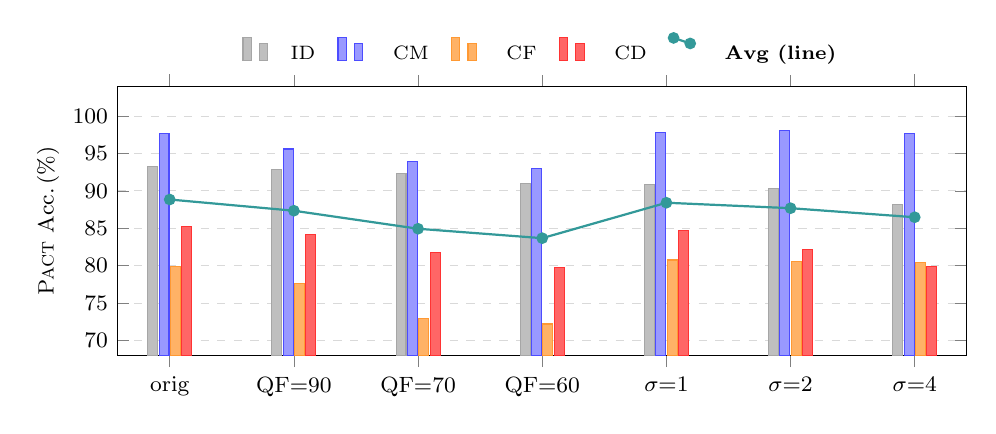
\begin{tikzpicture}
\begin{axis}[
    width=1.02\columnwidth,
    height=5.0cm,
    ybar=0.5pt,
    bar width=3.6pt,
    enlarge x limits=0.07,
    ymin=68, ymax=104,
    ytick={70,75,80,85,90,95,100},
    ymajorgrids=true,
    grid style={dashed,gray!30},
    ylabel={\vfive{} Acc.\,(\%)},
    ylabel style={font=\footnotesize,yshift=-2pt},
    symbolic x coords={orig,QF=90,QF=70,QF=60,$\sigma{=}1$,$\sigma{=}2$,$\sigma{=}4$},
    xtick=data,
    xticklabel style={font=\footnotesize},
    yticklabel style={font=\footnotesize},
    legend style={
        at={(0.5,1.04)}, anchor=south,
        legend columns=5,
        font=\scriptsize,
        draw=none,
        column sep=6pt,
    },
]
\addplot[fill=gray!50,draw=gray!70] coordinates {(orig,93.27) (QF=90,92.91) (QF=70,92.27) (QF=60,91.00) ($\sigma{=}1$,90.82) ($\sigma{=}2$,90.36) ($\sigma{=}4$,88.18)};
\addplot[fill=blue!40,draw=blue!70] coordinates {(orig,97.65) (QF=90,95.61) (QF=70,93.94) (QF=60,92.95) ($\sigma{=}1$,97.80) ($\sigma{=}2$,98.11) ($\sigma{=}4$,97.65)};
\addplot[fill=orange!60,draw=orange!80] coordinates {(orig,79.92) (QF=90,77.65) (QF=70,72.95) (QF=60,72.20) ($\sigma{=}1$,80.76) ($\sigma{=}2$,80.53) ($\sigma{=}4$,80.45)};
\addplot[fill=red!60,draw=red!80] coordinates {(orig,85.30) (QF=90,84.17) (QF=70,81.82) (QF=60,79.77) ($\sigma{=}1$,84.70) ($\sigma{=}2$,82.20) ($\sigma{=}4$,79.92)};
\addplot[teal!80,thick,sharp plot,update limits=false,mark=*,mark size=1.7pt] coordinates {(orig,88.85) (QF=90,87.35) (QF=70,84.94) (QF=60,83.68) ($\sigma{=}1$,88.42) ($\sigma{=}2$,87.69) ($\sigma{=}4$,86.48)};
\legend{ID,\ CM,\ CF,\ CD,\ \textbf{Avg (line)}}
\end{axis}
\end{tikzpicture}
\caption{\textbf{Robustness of \textsc{GenStack} to JPEG compression and Gaussian blur} per HydraFake split (ID gray, CM blue, CF orange, CD red) and the sample-weighted average (teal). The architecture stays above $83\%$ across all seven perturbation conditions, indicating it is robust to realistic post-processing. See \S\ref{sec:robustness_degrade} for analysis.}
\label{fig:robust_degrade}
\end{figure}

% \subsection{Limitations}
% \label{sec:limitations}

% GenStack has three limitations that shape natural directions for follow-up work. The learned gate routes inputs to one of the $|\mathcal{G}|{=}23$ HydraFake generators it was trained on; on a fully novel generator outside this vocabulary the gate falls back to the closest in-vocabulary match, costing $-3.29$ pp on average in the leave-one-generator-out study (\S\ref{sec:open_world}) and motivating periodic re-fitting as new generators emerge. The per-generator experts are trained with $5$-fold cross-validation within each generator's samples, which assumes access to per-generator labels at training time even though every reported number remains held-out. Finally, GenStack pairs two architecturally orthogonal bases (CLIP-based and MLLM-based); whether a third base can further close the cross-domain gap remains open.

% =====================================================================
% 5. Discussion
% =====================================================================
\section{Conclusion}
\label{sec:conclusion}
To summarize, this paper makes the following contributions. We introduce \textsc{GenStack}, a dual-branch detector that pairs a parameter-efficient CLIP-based discriminative branch (\vfive) with a multi-view MLLM reasoner (\prism) trained on RGB, frequency, and noise-residual views. We propose a label-free Mixture-of-Experts fusion stage with a learned soft gate over CLIP features, using only $K{=}15$ KMeans-cluster experts. On HydraFake, \textsc{GenStack} establishes a new state-of-the-art across $23$ generators and four generalization splits, with the largest gains on the cross-forgery and cross-domain regimes where prior detectors fall short, all without any reinforcement-learning stage. 

%%%%%%%%% REFERENCES
{\small
\bibliographystyle{ieee}
\bibliography{references}
}

\end{document}